\chapter{Performance Analysis}

The analyses presented in this chapter should be interpreted as exploratory rather than causal. Campaign cahracteristics including platform, product\_category, audience\_target, creative\_types, etc.. are not independently distributed across the dataset.

Consequently, observed performance differences cannot be attributed to any single factor in isolation. Instead, the objective of this chapter is to identify consistent performance patterns, prioritize areas for further investigation, and generate hypotheses to guide future optimization and controlled experiments.

However, descriptive statistics alone cannot determine whether these observed differences represent genuine performance differences or are simply the result of random variation. Therefore, statistical significance testing was performed before drawing business conclusions.

\section{Statistical Methodology}

The following statistical tests were used throughout the analysis:

\begin{enumerate}
	
	\item \textbf{Shapiro--Wilk Test}
	
	Used to assess whether the distribution of each performance metric follows a normal distribution. The results determined whether parametric statistical methods were appropriate for subsequent analyses.
	
	\textbf{Statistical Question:}
	\begin{itemize}
		\item \textit{Do the observed performance metrics satisfy the assumptions required for parametric statistical tests?}
	\end{itemize}
	
	\item \textbf{Levene's Test}
	
	Used to determine whether the variability (consistency) of a performance metric differs significantly across groups.
	
	\textbf{Business Question Answered:}
	\begin{itemize}
		\item \textit{Which business groups deliver more consistent advertising performance, and which exhibit greater variability or unpredictability?}
	\end{itemize}
	
	\item \textbf{Kruskal--Wallis Test}
	
	A non-parametric alternative to one-way ANOVA used to determine whether the distribution of a performance metric differs significantly across multiple groups. This test was selected because the normality assumption required for ANOVA was not satisfied.
	
	\textbf{Business Question Answered:}
	\begin{itemize}
		\item \textit{Do the observed differences in campaign performance across business groups (e.g., platforms, regions, creative types, product categories, and target audiences) represent genuine differences, or are they likely due to random variation?}
	\end{itemize}
	
	\item \textbf{Dunn's Post-hoc Test}
	
	Performed following a statistically significant Kruskal--Wallis test to identify which specific groups differ from one another while controlling for multiple comparisons.
	
	\textbf{Business Question Answered:}
	\begin{itemize}
		\item \textit{If significant differences exist, which specific business groups differ in their advertising performance?}
	\end{itemize}
	
\end{enumerate}

Together, these statistical procedures provide a systematic framework for validating assumptions, assessing performance consistency, determining whether differences are statistically significant, and identifying the specific groups responsible for those differences.

%%%%%%%%%%%%%%%%%%%%%%%%%%%%%%%%%%%%%%%%%%%%%%%%%%%%%%%%%%%%%%%%%%%%%%%%%%%%%%%%%%%%%%%%%%%%%%%%%%%%%%%%%%%%%%%%%%%%%%%%%%%%%%%%%%%%%%%%%%%%%%%%%%%%%%%%%%

\newpage
\section{Channel Performance Analysis}
Performance metrics across different channel/platforms was investigated and is shown in Fig. \ref{fig:metrics_by_platform}. 

\begin{figure}[h]
	\centering
	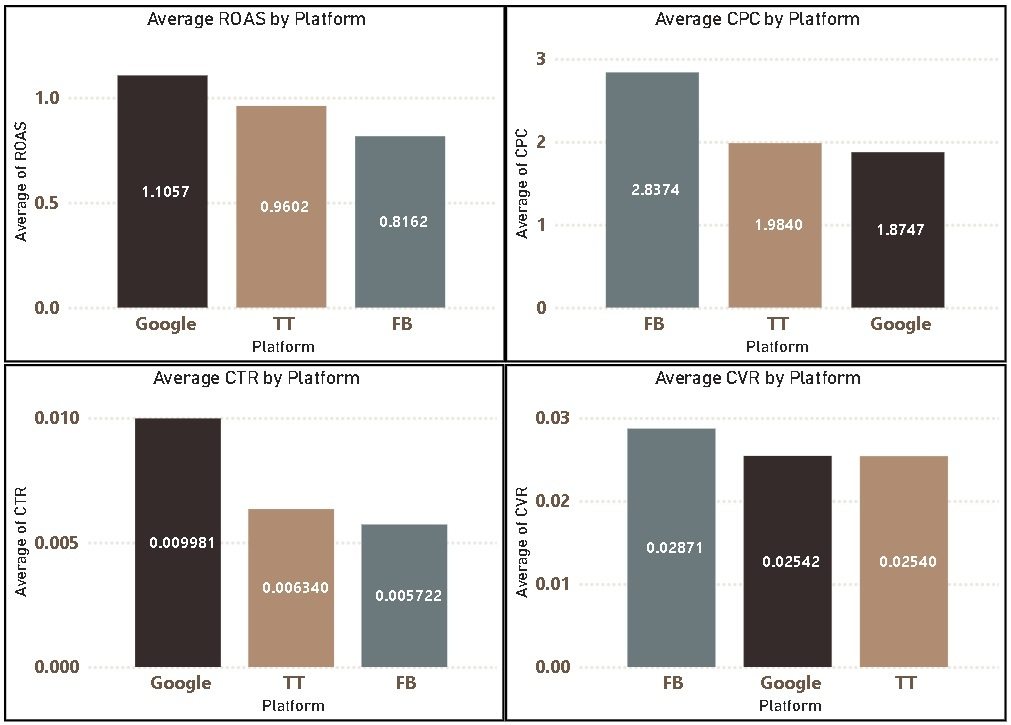
\includegraphics[width=1\textwidth]{images/metrics_by_platform.jpg}
	\caption{Performance Metrics by Platform}
	\label{fig:metrics_by_platform}
\end{figure}

\begin{itemize}
	\item FB exhibited the highest CVR out of all platforms which is offset by the high CPC and low CTR leading to its low ROAS.
	
	\item Google exhibited the highest CTR across platforms with the lowest Cost per Clicks.
	 
	\item From a business perspective, Google currently delivers the greatest overall value in contrast to FB platform based on their ROAS.
	
\end{itemize}

Drilling down on platforms by creative\_type we can see that Google search exhibited high ROAS while google Display exhibited one of the lowest ROAS as shown in Fig. \ref{fig:metrics_by_platform_creatives}. 

\begin{figure}[h]
	\centering
	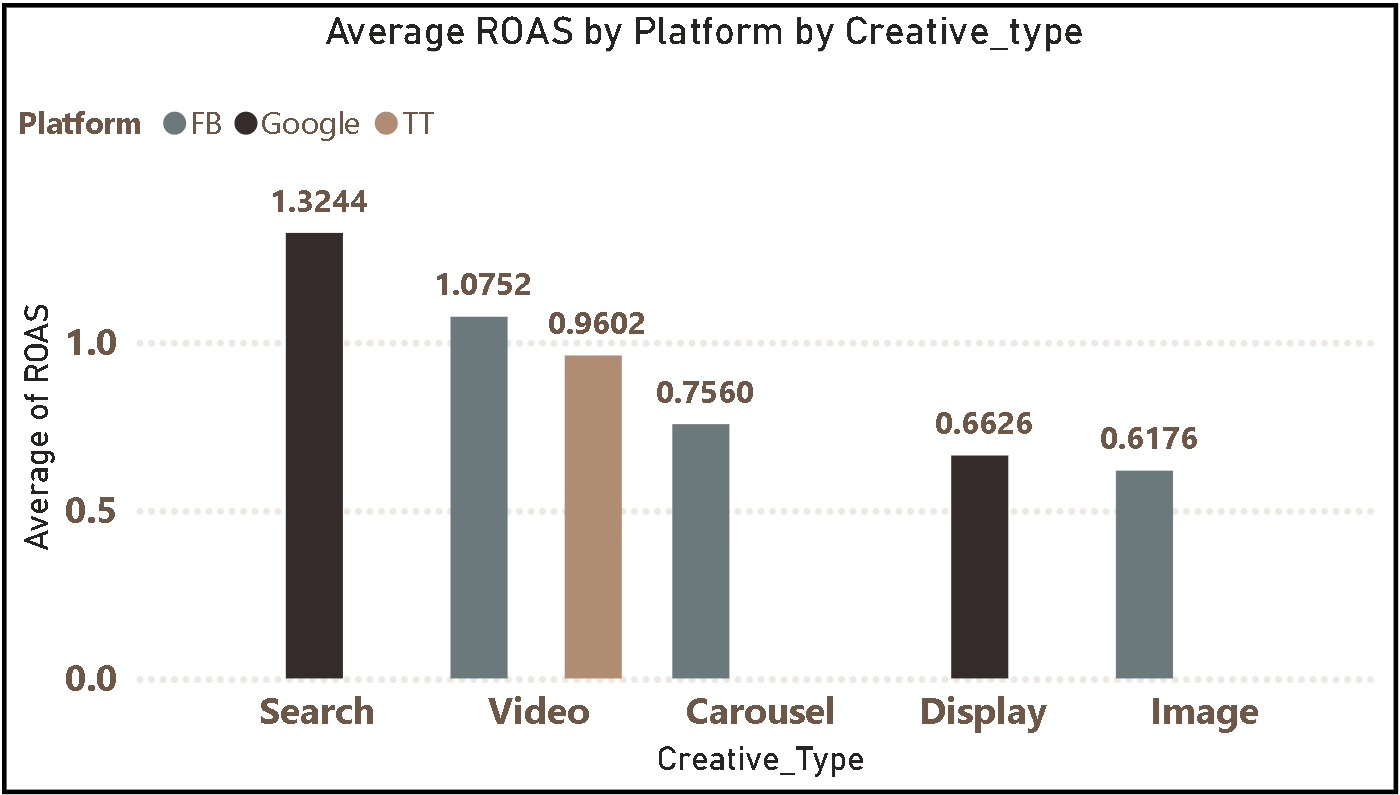
\includegraphics[width=0.6\textwidth]{images/ROAS_by_platform_by_creative.jpg}
	\caption{ROAS by Platform by Creative\_type}
	\label{fig:metrics_by_platform_creatives}
\end{figure}

This indicates that  \textbf{the performance of an ad campaign is not tied to the platform}, further analyses is required.
 
%%%%%%%%%%%%%%%%%%%%%%%%%%%%%%%%%%%%%%%%%%%%%%%%%%%%%%%%%%%%%%%%%%%%%%%%%%%%%%%%%%%%%%%%%%%%%%%%%%%%%%%%%%%%%%%%%%%%%%%%%%%%%%%%%%%%%%%%%%%%

\newpage
\section{Regional Performance Analysis}



\begin{figure}[h]
	\centering
	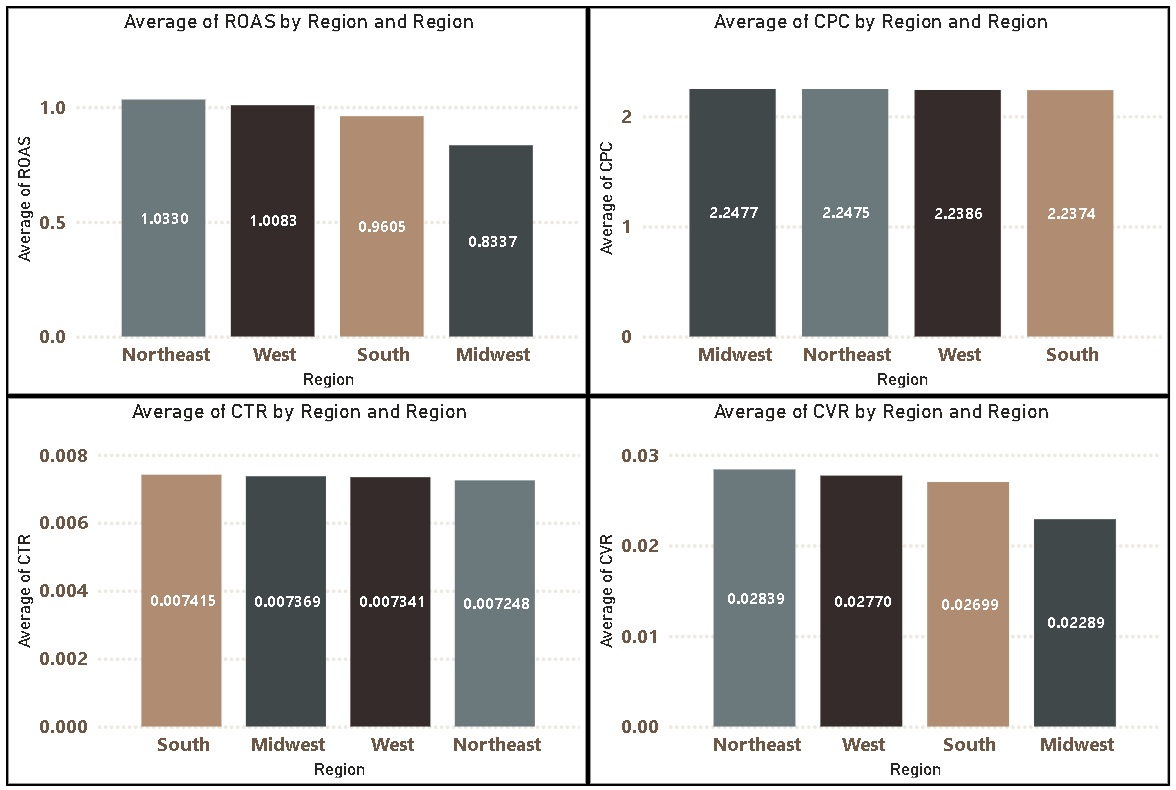
\includegraphics[width=0.8\textwidth]{images/metrics_by_region.jpg}
	\caption{Performance Metrics by Region}
	\label{fig:metrics_by_region}
\end{figure}



\begin{itemize}

	
	\item The \textbf{Midwest} consistently underperformed, recording both the lowest ROAS and the lowest conversion rate despite exhibiting click-through rates comparable to the other regions. This suggests that the primary challenge lies in converting interested users into customers rather than attracting engagement in this region.
	
	\item Because CTR and CPC did not differ significantly across regions, regional performance differences appear to be driven primarily by post-click behavior rather than differences in advertising cost or user engagement.
	

\end{itemize}




From a business perspective, further investigation should focus on \textbf{identifying factors that contribute to the Midwest's weaker conversion performance}. 

Potential explanations include regional differences in customer preferences, purchasing behavior, market competition, or campaign targeting strategies.


%%%%%%%%%%%%%%%%%%%%%%%%%%%%%%%%%%%%%%%%%%%%%%%%%%%%%%%%%%%%%%%%%%%%%%%%%%%%%%%%%%%%%%%%%%%%%%%%%%%%%%%%%%%%%%%%%%%%%%%%%%%%%%%%%%%%%%%%%%%%


\newpage
\section{Creative Performance Analysis}
Creative formats are highly imbalanced across campaigns, with certain creative types represented by only one or two campaigns as shown in Fig. \ref{fig:creative_type_count}. Consequently, comparisons should be interpreted as descriptive rather than causal.  

\begin{figure}[H]
	\centering
	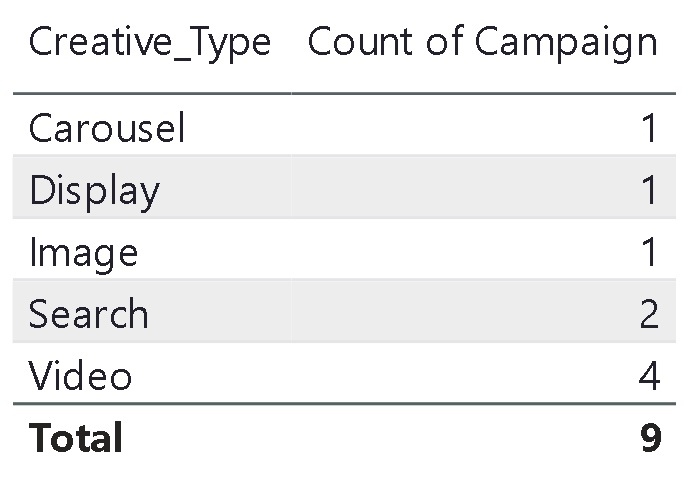
\includegraphics[width=0.3\textwidth]{images/creative_type_count.jpg}
	\caption{Creative Type Campaign counts}
	\label{fig:creative_type_count}
\end{figure}

Accordingly, the following observations are intended to describe aggregate performance patterns rather than isolate the causal effect of creative format. 

\begin{figure}[H]
	\centering
	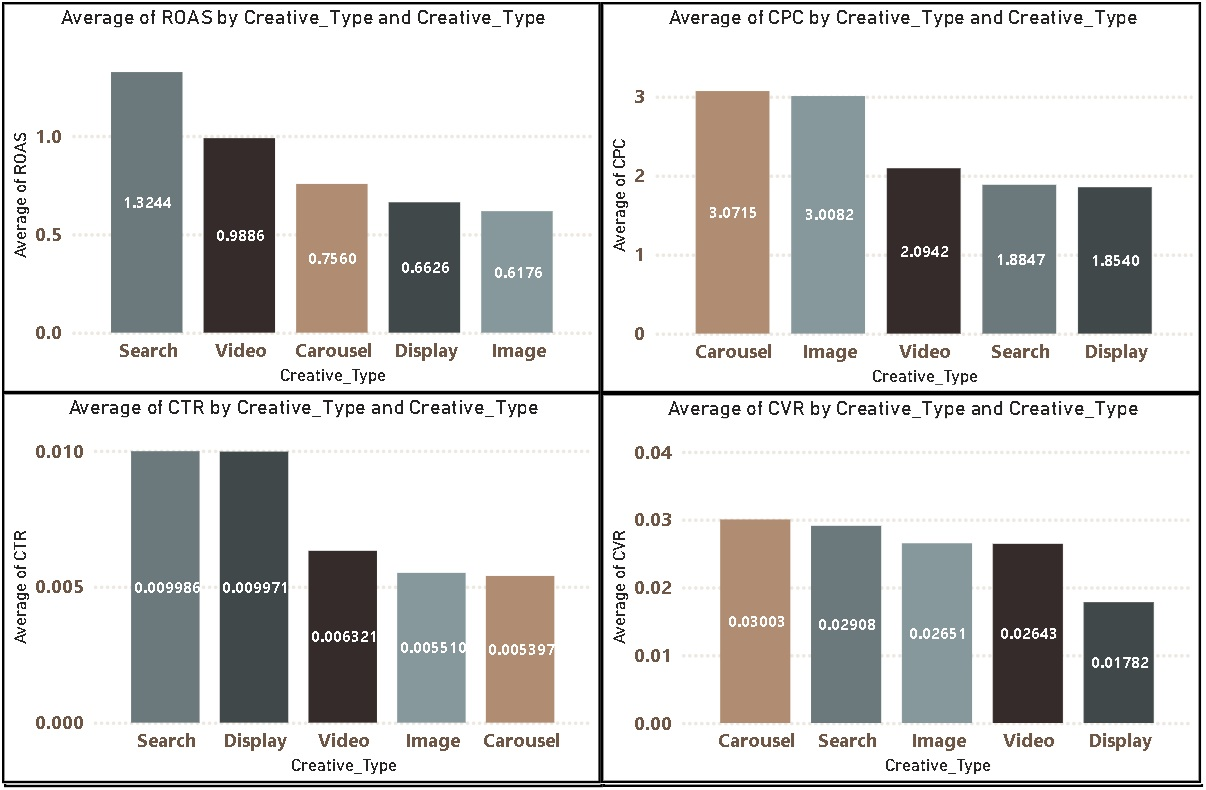
\includegraphics[width=0.8\textwidth]{images/metrics_by_creative.jpg}
	\caption{Performance Metrics by Creatives}
	\label{fig:metrics_by_creatives}
\end{figure}

Statistical significance tests for this section is shown in detail in Appendix \ref{appendix:creative_performance_analysis}. 
\begin{itemize}
	\item Search creatives exhibited the highest ROAS, whereas Display and Image exhibited the lowest ROAS.
	\item Search and Display successfuly generate clicks as shown by their CTR.
	\item In terms of traffic acquisition cost, carousel and image creatives are the most expensive.
	\item Carousel and Search exhibit the highest conversion efficiency as evidenced by their high CVR.
\end{itemize}

\subsection{Video Completion Rate vs Conversion}
We explored the relationship between video completion rate and conversion efficiency(CVR) as shown in Fig. \ref{fig:video_completion_rate}.


\begin{figure}[H]
	\centering
	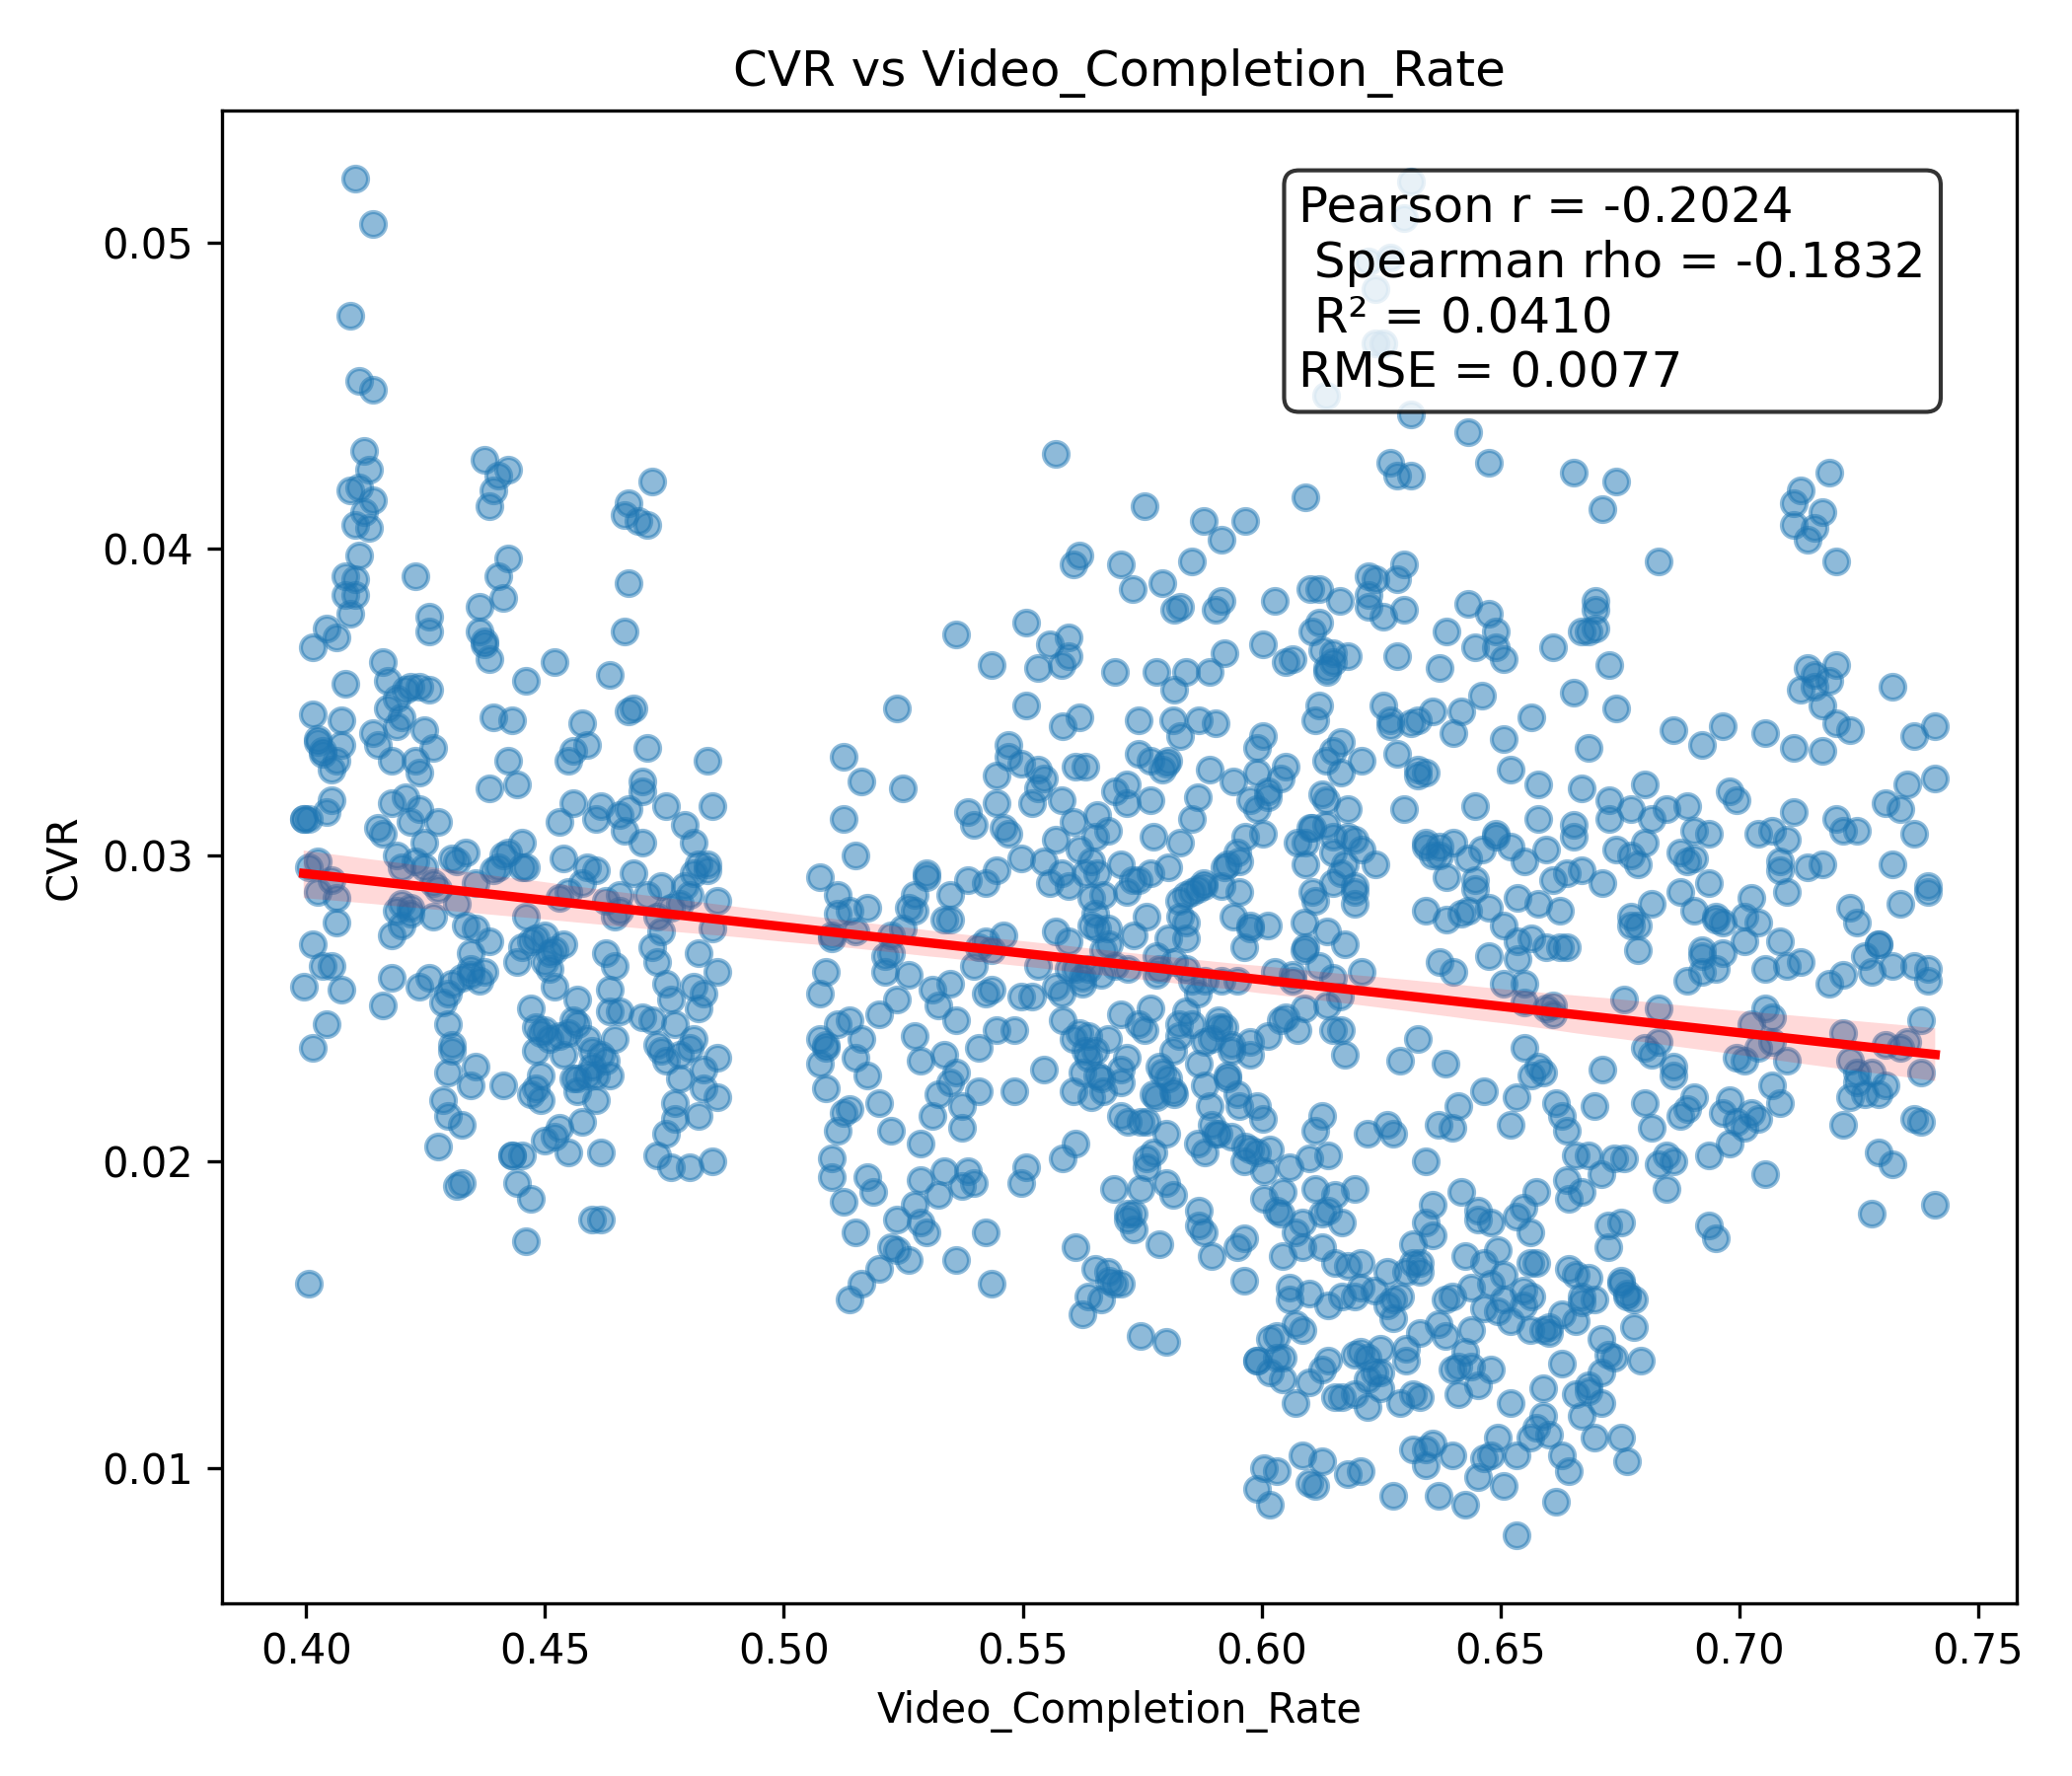
\includegraphics[width=0.7\textwidth]{images/CVR_vs_Video_Completion_Rate.png}
	\caption{CVR vs Video Completion Rate}
	\label{fig:video_completion_rate}
\end{figure}

There is no statistically significant correlation between the conversion rate(CVR) and video completion rate. 












	
	
	
%%%%%%%%%%%%%%%%%%%%%%%%%%%%%%%%%%%%%%%%%%%%%%%%%%%%%%%%%%%%%%%%%%%%%%%%%%%%%%%%%%%%%%%%%%%%%%%%%%%%%%%%%%%%%%%%%%%%%%
\section{Audience-Product Performance Analysis}
Performance of existing campaigns across different audience-product pairs was also investigated. 

\begin{figure}[H]
	\centering
	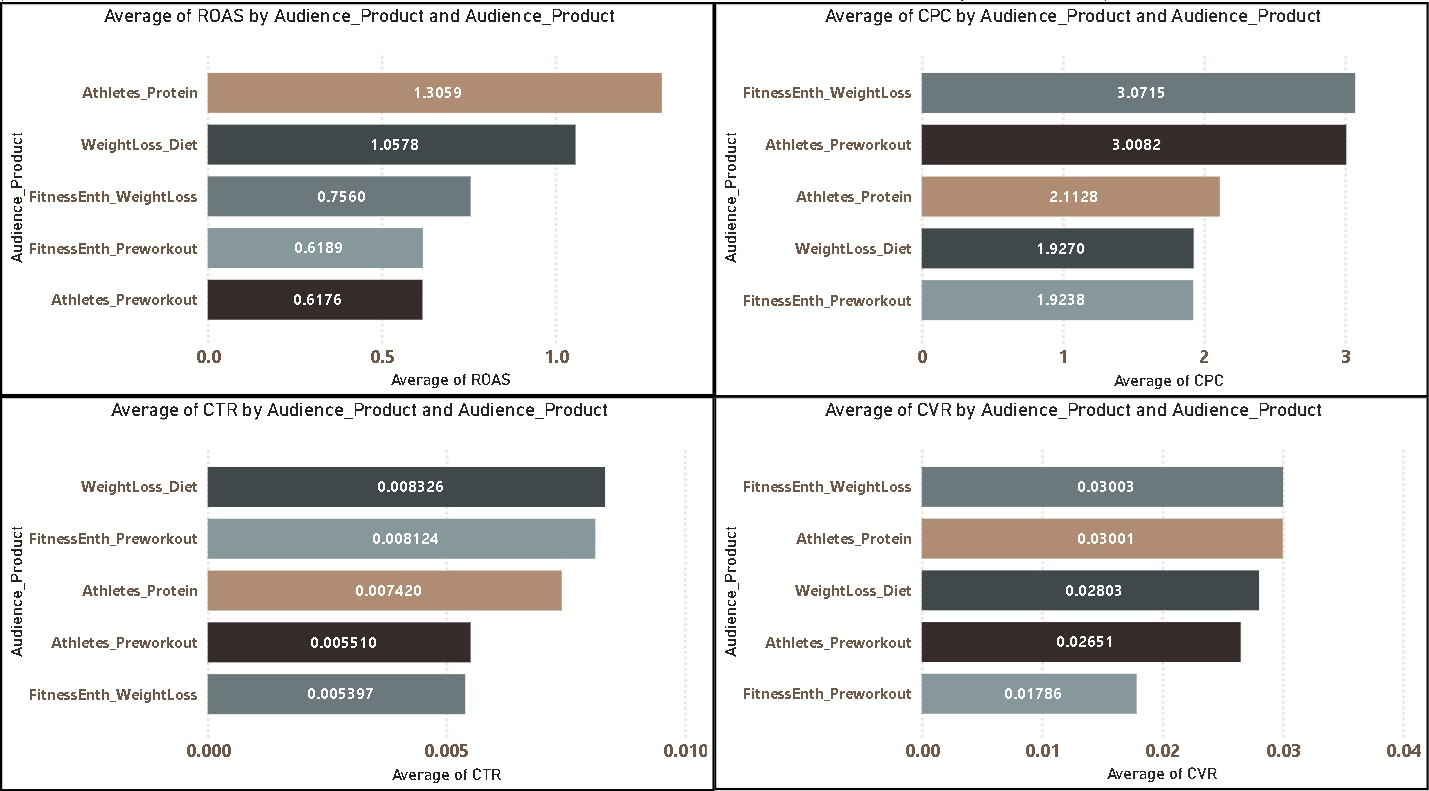
\includegraphics[width=1\textwidth]{images/metrics_by_audience-product.jpg}
	\caption{Performance Metrics by Audience-Product}
	\label{fig:audience-product}
\end{figure}

\begin{itemize}
	
	\item The \textbf{Athletes-Protein} combination demonstrated the strongest overall performance, achieving the highest ROAS while maintaining one of the highest conversion rates. This audience-product pairing appears to generate the greatest financial return from advertising investment.
	
	\item The \textbf{WeightLoss-Diet} combination also performed strongly, producing the second-highest ROAS, the highest click-through rate, and relatively low acquisition costs. These findings suggest that Diet campaigns are particularly effective when targeted toward individuals interested in weight loss.
	
	\item Both \textbf{Athletes-Preworkout} and \textbf{FitnessEnth-Preworkout} consistently exhibited poor ROAS despite differing levels of user engagement. This suggests that the weak financial performance of Pre-workout campaigns is not driven solely by audience selection, but may instead reflect broader issues related to the product offering, campaign messaging, pricing strategy, or post-click conversion experience.
	
	\item The \textbf{FitnessEnth-WeightLoss} combination achieved one of the highest conversion rates but also incurred the highest advertising cost per click. Although this audience converts effectively, its relatively high acquisition cost reduces overall profitability.
	
	\item Because statistically significant differences were observed across all four performance metrics, optimizing campaign performance should consider the \textbf{audience--product pairing} rather than treating audience and product category as independent marketing decisions.
	
\end{itemize}

From a business perspective, these findings suggest that future optimization efforts should evaluate the effectiveness of specific audience--product combinations rather than optimizing audience targeting or product campaigns independently. For example, investigating why the \textbf{WeightLoss--Diet} and \textbf{Athletes--Protein} pairings consistently outperform other combinations may reveal successful strategies that can be applied to other campaigns. Likewise, the consistently poor performance of both \textbf{Pre-workout} audience pairings suggests that improving audience selection alone is unlikely to substantially increase profitability. Instead, optimization should focus on the entire campaign strategy surrounding these pairings, including product positioning, promotional messaging, pricing, and landing page experience.


%%%%%%%%%%%%%%%%%%%%%%%%%%%%%%%%%%%%%%%%%%%%%%%%%%%%%%%%%%%%%%%%%%%%%%%%%%%%%%%%%%%%%%%%%%%%%%%%%%%%%%%%%%%%%%%%%%%%%%





%%%%%%%%%%%%%%%%%%%%%%%%%%%%%%%%%%%%%%%%%%%%%%%%%%%%%%%%%%%%%%%%%%%%%%%%%%%%%%%%%%%%%%%%%%%%%%%%%%%%%%%%%%%%%%%%%%%%%%

\section{Effect of Competitive Events}

The exploratory assessment examined whether campaign performance differed during periods with and without competitive events.

A complete summary of the statistical analyses, including assumption checks, Kruskal--Wallis tests, and pairwise comparisons, is provided in Appendix~\ref{appendix:competitive_event_performance_analysis}.

\begin{figure}[h]
	\centering
	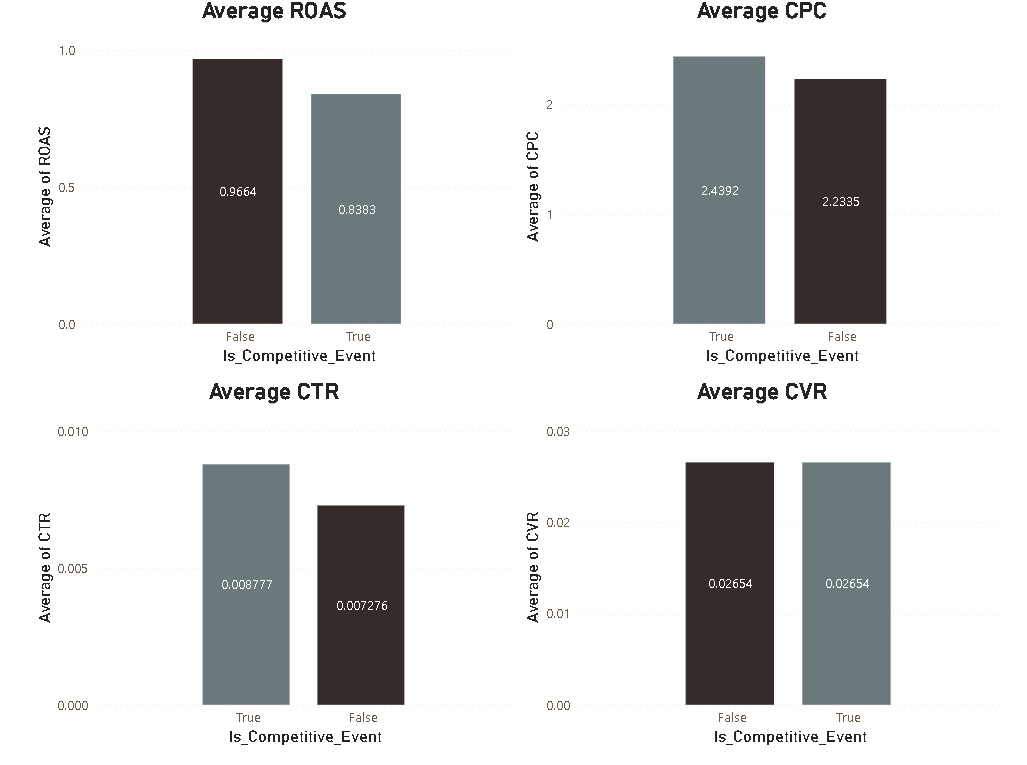
\includegraphics[width=\textwidth]{images/competitive_event_effect.jpg}
	\caption{Comparison of campaign performance during competitive and non-competitive periods.}
	\label{fig:competitive_event_summary}
\end{figure}

Figure~\ref{fig:competitive_event_summary} summarizes the influence of competitive events on the four primary advertising performance metrics.

Campaigns conducted during competitive events achieved a significantly lower average ROAS (0.838) than campaigns conducted outside competitive periods (0.966), indicating reduced advertising profitability (Appendix~\ref{appendix:competitive_event_performance_analysis_ROAS}).

Interestingly, campaigns during competitive events generated significantly higher CTR (0.88\% versus 0.73\%), suggesting that advertisements attracted greater user engagement despite increased market competition (Appendix~\ref{appendix:competitive_event_performance_analysis_CTR}).

However, this increase in engagement did not translate into improved purchasing behavior. Conversion rates remained statistically unchanged between competitive and non-competitive periods (approximately 2.65\%), indicating that users who clicked advertisements were equally likely to complete a purchase regardless of competitive conditions (Appendix~\ref{appendix:competitive_event_performance_analysis_CVR}).

Competitive events were also associated with significantly higher CPC (\$2.44 versus \$2.23), indicating that advertisers paid more to acquire each click (Appendix~\ref{appendix:competitive_event_performance_analysis_CPC}).

Taken together, these findings suggest that competitive events primarily reduce campaign profitability by increasing advertising costs rather than by reducing customer purchase intent. Although advertisements attracted more clicks during competitive periods, the higher acquisition cost combined with unchanged conversion performance resulted in significantly lower ROAS.

From a business perspective, campaigns scheduled during competitive periods may require stronger creative assets, more precise audience targeting, or more compelling promotional offers to justify the higher advertising costs. Alternatively, campaigns focused primarily on maximizing profitability may benefit from allocating a larger portion of the advertising budget to less competitive periods where comparable conversion rates can be achieved at lower acquisition costs.


\section{Temporal Analysis}

